\begin{frame}{Процессы. Общая информация}
\begin{columns}
        \column{0.8\textwidth}
  \begin{block}{Процесс}
    \begin{itemize}
      \item Данные с диска загружаются в оперативную память.
      \item Процесс состоит из инструкций, выполняемых процессором, данных и информации о выполняемой задаче 
      \item Программа запускает 1 или более процессов. 
    \end{itemize} 
  \end{block}
  \begin{block}{Изоляция процессов}
    \begin{itemize}
      \item Процессы изолированы друг от друга\footnote{нет доступа к памяти и стеку, открытым файлам и порядку выполения}.
      \item Для обмена данными используется система межпроцессного взаимодействия (IPC)
      \item Следствие: пользователи могут запускать несколько экземпляров одной и той же программы. 
    \end{itemize}
  \end{block}
        \column{0.3\textwidth}
        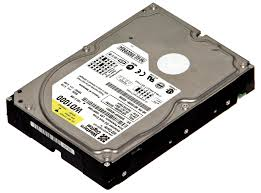
\includegraphics[height=2cm]{hw_hdd.jpg} \break
        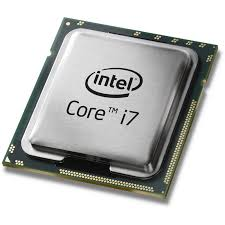
\includegraphics[height=2cm]{hw_cpu.jpg} \break
        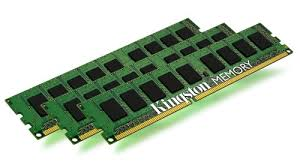
\includegraphics[height=2cm]{hw_memory.jpg} 
\end{columns}
\end{frame}


